
\documentclass{beamer}

%\usepackage[table]{xcolor}
\mode<presentation> {
  \usetheme{Boadilla}

%  \usetheme{Pittsburgh}
%\usefonttheme[2]{sans}
\renewcommand{\familydefault}{cmss}
%\usepackage{lmodern}
%\usepackage[T1]{fontenc}
%\usepackage{palatino}
%\usepackage{cmbright}
  \setbeamercovered{transparent}
\useinnertheme{rectangles}
}

\setbeamercolor{normal text}{fg=black}
\setbeamercolor{structure}{fg= blue}
\definecolor{trial}{cmyk}{1,0,0, 0}
\definecolor{trial2}{cmyk}{0.00,0,1, 0}
\definecolor{darkgreen}{rgb}{0,.4, 0.1}
\usepackage{array}
\beamertemplatesolidbackgroundcolor{white}  \setbeamercolor{alerted
text}{fg=red}
\usepackage{tcolorbox}
\setbeamertemplate{caption}[numbered]\newcounter{mylastframe}


\usepackage{tikz}
\usetikzlibrary{arrows}
\usepackage{colortbl}

\renewcommand{\familydefault}{cmss}
%\usepackage[all]{xy}

\usepackage{tikz}
\usepackage{lipsum}

 \newenvironment{changemargin}[3]{%
 \begin{list}{}{%
 \setlength{\topsep}{0pt}%
 \setlength{\leftmargin}{#1}%
 \setlength{\rightmargin}{#2}%
 \setlength{\topmargin}{#3}%
 \setlength{\listparindent}{\parindent}%
 \setlength{\itemindent}{\parindent}%
 \setlength{\parsep}{\parskip}%
 }%
\item[]}{\end{list}}
\usetikzlibrary{arrows}

\usecolortheme{lily}

\newtheorem{com}{Comment}
\newtheorem{lem} {Lemma}
\newtheorem{prop}{Proposition}
\newtheorem{condition}{Condition}
\newtheorem{thm}{Theorem}
\newtheorem{defn}{Definition}
\newtheorem{cor}{Corollary}
\newtheorem{obs}{Observation}
 \numberwithin{equation}{section}
 

\setbeamertemplate{navigation symbols}{}


\title[PLSC 43401]{Mathematical Foundations of Political Methodology}

\author{Robert Gulotty}
\institute[Chicago]{University of Chicago}
\vspace{0.3in}




\begin{document}




\begin{frame}
\maketitle
\end{frame}



\begin{frame}
\frametitle{Interpreting Causal Effects}

Rubin Causal Model: \pause 
\begin{itemize}
\invisible<1>{\item[-] $Y_{i}(1)$: response under treatment} \pause 
\invisible<1-2>{\item[-] $Y_{i}(0)$: response under control } \pause 
\end{itemize}
\invisible<1-3>{Individual Treatment Effect: $Y_{i}(1) - Y_{i}(0)$} \pause  \\
\invisible<1-4>{Fundamental problem of causal inference:}\pause \\
\only<1-6>{\invisible<1-5>{$Y_{i}(1) - Y_{i}(0)$}} \pause
\only<7->{\invisible<8>{$Y_{i}(1)$} - \invisible<1-7>{$Y_{i}(0)$}} \pause \pause \pause \\
\invisible<1-9>{ATE $= E[Y(1) - Y(0)]$ } 




\end{frame}






\begin{frame}
\frametitle{Observational Studies and Causal Inference}


\alert{Experimental} studies:\pause 
\begin{itemize}
\invisible<1>{\item[-] Treatment under control of analyst} 
\invisible<1>{\item[-] Random assignment, estimate
\begin{eqnarray}
\widehat{ATE} = E[Y(1)| T = 1] - E[Y(0) | T=0] \nonumber.\pause 
\end{eqnarray}
Because $E[Y(1)] = E[Y(1)|T= 1] = \alert{E[Y(1)| T = 0]} $ and $E[Y(0)] = E[Y(0)|T= 0] = \alert{E[Y(0)| T = 1]} $

}  \pause 
\end{itemize}
\invisible<1-2>{\alert{Observational} } \pause 
\begin{itemize}
\invisible<1-3>{\item[-] Units (people, countries) control their treatment status} \pause 
\invisible<1-4>{\item[-] \alert{Selection}: treatment and control groups differ systematically} \pause 
\begin{itemize}
\invisible<1-5>{\item[-] $E[Y(1)|T=1] \neq E[Y(1) |T = 0] $, $[EY(0)|T =0 ] \neq E[Y(0)|T = 1] $} \pause 
\invisible<1-6>{\item[-] Observables: things we can see, measure, and use in our study} \pause 
\invisible<1-7>{\item[-] Unobservables: not observables (big problem)} \pause 
\end{itemize}
\invisible<1-8>{\item[-]  Naive difference in means will be biased} \pause 
\invisible<1-9>{\item[-] Many, many, potential strategies for limiting bias} \pause 
\invisible<1-10>{\item[-] \alert{Regression is just one method}} 
\end{itemize}



\end{frame}


\begin{frame}
\frametitle{The Problem of Selection} 

\begin{eqnarray} 
\text{ATE} &= & E[Y(1) - Y(0) ] \nonumber  \pause \\
\invisible<1>{& = & E[Y(1)] - E[Y(0) ] \nonumber } \pause \\
\invisible<1-2>{ & =& \{\alert{E[Y(1) | T = 1]}  \alert{Pr(T= 1)} + \textcolor{blue}{E[Y(1) | T = 0 ]}  \alert{Pr(T = 0 )} \}   \nonumber \\
 & &- \{ \alert{E[Y(0) | T= 0 ] Pr(T =0 )} +  \textcolor{blue}{E[Y(0) | T=1]} \alert{Pr(T = 1)} \} \nonumber } \pause 
\end{eqnarray}
\end{frame}

\begin{frame}
\frametitle{Manski Bound} 

What can we learn in the face of selection?  \pause \\
\invisible<1>{Suppose that we have a dichotomous dependent variable } \pause 
\begin{itemize}
\invisible<1-2>{\item[-] Smallest ATE: $-1$ } \pause 
\invisible<1-3>{\item[-] Largest ATE: $1$} \pause 
\invisible<1-4>{\item[-] Length: $2$ } \pause 
\invisible<1-5>{\item[-] $-1< ATE<1$} \pause 
\end{itemize}
\invisible<1-6>{\alert{Manksi Bounds}: \\} \pause 
\begin{itemize}
\invisible<1-7>{\item[-] Interval that contains true ATE with probability 1} \pause 
\invisible<1-8>{\item[-] Reduces interval length to $1$ } \pause 
\invisible<1-9>{\item[-] \alert{Requires no additional assumptions} } 
\end{itemize}


\end{frame}

\begin{frame}
\frametitle{Manski Bound} 
Note that: \\
$0\leq E[Y(1) | T = 0 ] \leq 1$ \pause \\
\invisible<1>{And that: \\
$0 \leq E[Y(0)| T=1] \leq 1$} \pause 

\invisible<1-2>{And recall that, } \pause 
\footnotesize
\begin{eqnarray}
\invisible<1-3>{ATE & =& \{\alert{E[Y(1) | T = 1]}  \alert{Pr(T= 1)} + \textcolor{blue}{E[Y(1) | T = 0 ]}  \alert{Pr(T = 0 )} \}   \nonumber \\
 & &- \{ \alert{E[Y(0) | T= 0 ] Pr(T =0 )} +  \textcolor{blue}{E[Y(0) | T=1]} \alert{Pr(T = 1)} \} \nonumber \\
 & = & \alert{E[Y(1) | T = 1] \pi} + \textcolor{blue}{E[Y(1) | T = 0 ]} \alert{(1- \pi)} \nonumber \\
 & & - \alert{E[Y(0) | T= 0 ] (1- \pi)} - \textcolor{blue}{E[Y(0) | T=1]}\alert{\pi} \nonumber } \pause 
 \end{eqnarray}
\invisible<1-4>{So, we can form bounds } \pause 
\begin{eqnarray} 
\invisible<1-5>{E[Y(1)|T=1] \pi -  (1-\pi) E[Y(0)| T= 0] - \pi } & & \nonumber  \\
\invisible<1-5>{<  ATE} \pause \invisible<1-6>{  < & & \nonumber \\
 E[Y(1)|T= ] \pi - (1-\pi) E[Y(0)| T= 0] + 1 - \pi   } & &\nonumber 
\end{eqnarray} 

\end{frame}

\begin{frame}
\frametitle{Manski Bound} 

The Manski bound \pause \\
\invisible<1>{$[\text{Average(Treat)} \pi -  (1-\pi) \text{Average(Control)}- \pi , $\\
\hspace{1in} $\text{Average(Treat)}\pi -  (1-\pi) \text{Average(Control)} + 1 - \pi ]$\\
 and has length $1$.  }\pause 


\invisible<1-2>{From Keele 2009: Presidential Visits + Congressional Wins} \pause 
\begin{itemize}
\invisible<1-3>{\item[-] $\pi = 0.06$} \pause 
\invisible<1-4>{\item[-] $E[Y(1)|T=1] = 18/21 = 0.857$} \pause 
\invisible<1-5>{\item[-] $E[Y(0)|T = 0] = 163/(327) =0.498$} \pause 
\end{itemize}
\invisible<1-6>{Bound is then:} \pause 
\begin{eqnarray}
\invisible<1-7>{&&[0.86\times 0.06 - 0.94\times 0.498 - 0.06  \textbf{,}  0.86\times 0.06 - 0.94\times 0.498 + 0.94] \nonumber \\
&&[-0.476  ,  0.523 ] \nonumber } \pause 
\end{eqnarray}



\begin{itemize}
\invisible<1-8>{\item[-] Further assumptions can narrow bounds} \pause 
\invisible<1-9>{\item[-] \alert{Law of Decreasing Credibility}: the credibility of inference decreases with the strength of the assumptions maintained} 
\end{itemize} 


\end{frame}

\begin{frame}
\frametitle{Causal Inference Via Stratification} 

Selection on observables:\pause 
\begin{itemize}
\invisible<1>{\item[-] Suppose that treatment is systematically related to outcomes (not ignorable) } \pause 
\begin{itemize}
\invisible<1-2>{\item[-] $E[Y(1)|D=1] \neq E[Y(1)|D =0]$ } \pause 
\invisible<1-3>{\item[-] $E[Y(0)|D=1] \neq E[Y(0)|D =0] $} \pause 
\invisible<1-4>{\item[-] Implies that Naive difference is not an unbiased estimate of ATE.  } \pause 
\end{itemize}
\invisible<1-5>{\item[-] Suppose there exists dichotomous variable $S$ such that,} \pause 
\begin{itemize}
\invisible<1-6>{\item[1)] $E[Y(1)|D=1, S]  =  E[Y(1)|D =0, S]$ } \pause 
\invisible<1-7>{\item[2)]  $E[Y(0)|D=1, S]  =  E[Y(0)|D =0, S] $} \pause 
\end{itemize}
\end{itemize}

\invisible<1-8>{\begin{prop} 
Suppose there exists $S$ such that $1)$ and $2)$ hold.  Then, we can obtain unbiased estimates for 
\begin{itemize}
\item[1)] $E[ATE|S=1] \equiv$ ATE, Given $S = 1$
\item[2)] $E[ATE|S =0] \equiv$ ATE, Given $S = 0$
\item[3)] ATE
\end{itemize}
\end{prop}}

\end{frame}

\begin{frame}
Idea: \pause 
\begin{itemize}
\invisible<1>{\item[1)] Average Treatment effect with strata, $S=1$} \pause 
\begin{itemize}
\invisible<1-2>{\item[-] Average(Treatment) - Average(Control) , for all units with $S=1$} \pause 
\end{itemize}
\invisible<1-3>{\item[2)] Average Treatment effect with strata, $S=0$} \pause 
\begin{itemize}
\invisible<1-4>{\item[-] Average(Treatment) - Average(Control) , for all units with $S=0$} \pause 
\end{itemize}
\invisible<1-5>{\item[3)] Average Treatment Effect} \pause 
\begin{itemize}
\invisible<1-6>{\item[-] Calculate Average(Treatment) - Average(Control) within each strata, $E[ATE|S]$} \pause 
\invisible<1-7>{\item[-] $ATE = \sum_{s=0}^{1} E[ATE|S]\times Pr(S) $} 
\end{itemize}
\end{itemize}

\end{frame}



\begin{frame}

\frametitle{Proof}
$E[Y(1)|S =1, D=1 ] - E[Y(0) | S=1, D= 0 ]$\pause 
\begin{eqnarray}
 \invisible<1>{& = & \{\text{Pr}(D=1|S=1)E[Y(1)|S=1, D=1] \nonumber \\
 & &+  \text{Pr}(D=0|S=1) E[Y(1)|S=1, D=1] \}\nonumber \\
& &-  \{\text{Pr}(D=1|S=1) E[Y(0)|S=1, D=0] \nonumber \\
&  &+   \text{Pr}(D=0|S=1) E[Y(0)| S= 1, D= 0 ] \} \nonumber \\} \pause 
\invisible<1-2>{ & = & \{\text{Pr}(D=1|S=1)E[Y(1)|S=1, D=1] \nonumber \\
 & &+  \text{Pr}(D=0|S=1) E[Y(1)|S=1, D=0] \}\nonumber \\
& &-  \{\text{Pr}(D=1|S=1) E[Y(0)|S=1, D=1] \nonumber \\
&  &+   \text{Pr}(D=0|S=1) E[Y(0)| S= 1, D= 0 ] \} \nonumber \\} \pause 
\invisible<1-3>{& = & E[ATE|S=1] \nonumber } 
\end{eqnarray}

\end{frame}







\begin{frame}
\frametitle{Causal Inference via Stratification: Example}

We are interested in the causal effect of \alert{incumbency} on reelection.  \\
\begin{itemize}
\item[-] $T=1$, Incumbent
\item[-] $T= 0$, Challenger
\end{itemize}
$Y_{i}(T)$ result of election. \\
Incumbency obviously not assigned at random.   \\
But suppose we have a dichotomous measure of candidate quality 
\begin{itemize}
\item[-] $S=1$, High quality
\item[-] $S=0$, Low quality
\end{itemize}
And that incumbency is as good as random, given $S$.  \\
We're interested in obtaining
\begin{eqnarray}
ATE & = & E[Y(1) - Y(0) ] \nonumber 
\end{eqnarray}

What if we don't condition on candidate quality?


\end{frame}

\begin{frame}

Joint Distribution of Treat and Strata

\small
\begin{tabular}{c|c|c|c}
\hline
 & T = 1 & T = 0 &  P(S)\\
 \hline
 S = 1 & 0.4 & 0.2 & 0.6 \\
 \hline
 S = 0 & 0.1 & 0.3 & 0.4 \\
 \hline
P(T) & 0.5  & 0.5 & \\
\hline 
\end{tabular}
\pause 

\invisible<1>{Potential Outcomes} \pause 
\invisible<1-2>{\begin{tabular}{c|c|c|c}
 & Control & Treat & ATE$|S$ \\
 \hline
 S = 1 &  $E[Y(0)|S = 1 ]$ = 0.5 & $E[Y(1)|S = 1]$ = 0.7 & 0.2 \\
 \hline
 S = 0 & $E[Y(0) | S= 0 ]$ = 0.38 & $E[Y(1)| S = 0 ]$= 0.4 & 0.02 \\
 \end{tabular}} \pause 
 \footnotesize
 
\invisible<1-3>{True $ATE$  = $0.2 \times 0.6 + 0.02 \times 0.4$ = \textcolor{blue}{0.128} } \pause \\
\invisible<1-4>{Naive difference in means: } \pause 
\begin{eqnarray}
\invisible<1-5>{E[Y(1)|T= 1] & = & 0.7 \times P(S=1|T=1) \nonumber \\
 & & + 0.4 \times P(S=0 | T= 1) \nonumber \\} \pause 
 \invisible<1-6>{& = & 0.7 \times \frac{4}{5} + 0.4 \times \frac{1}{5} = \alert{0.64} \nonumber \\} \pause 
\invisible<1-7>{ E[Y(0)|T= 0] & =& 0.5 \times \frac{2}{5} + 0.3\times\frac{3}{5} = \alert{0.38} \nonumber \\} \pause 
\invisible<1-8>{ E[Y(1)|T=1] - E[Y(0)|T= 0] & =& 0.64 - 0.38 \nonumber \\} \pause 
\invisible<1-9>{  & =& \alert{0.26} \nonumber } \pause
\end{eqnarray}


\invisible<1-10>{\alert{Why?}: those with bigger treatment effects more likely to select into treatment \\} \pause 
\invisible<1-11>{\alert{Confound} effect of $T$ with differences across $S$}
\end{frame}


\begin{frame}
\frametitle{With Stratification}
\pause 
\begin{eqnarray}
\invisible<1>{E[Y(1)|T=1, S= 1]  & = & 0.7 \nonumber \\
E[Y(0)|T=0, S =1] & = & 0.5 \nonumber \\
E[Y(1)|T =1, S= 0] & = & 0.4 \nonumber \\
E[Y(0)|T =0 , S =0 ] & = & 0.38 \nonumber } \pause 
\end{eqnarray}
\invisible<1-2>{$ \sum_{i=1}^{2}\left(E[Y(1)|S=i, T=1]  - E[Y(0)|S=i, T=0]\right) \text{Pr}(S=i) = $  \\} \pause 
\invisible<1-3>{$\left(0.7 - 0.5\right) \times 0.6  + \left(0.4 - 0.38\right)\times 0.4 = \alert{0.128}$} 
\end{frame}


\begin{frame}
\frametitle{Stratification and Matching}

Exact stratification is \alert{Exact Matching} \pause \\
\invisible<1>{Exact Matching, Basic idea: } \pause 
\begin{itemize}
\invisible<1-2>{\item[-] Identify all \alert{characteristics} (covariates) that affect both outcome and treatment assignment} \pause 
\invisible<1-3>{\item[-] For all treated units, identify \alert{control} unit with same characteristics} \pause 
\invisible<1-4>{\item[-] Exact match: units in the same strata} 
\end{itemize}

\end{frame}


\begin{frame}
\frametitle{What do we do?}

\alert{Most strata are empty, or only a few observations}
\begin{itemize}
\item[-] \alert{Bias}-\alert{Variance} tradeoff
\begin{itemize}
\item[-] Bias: assume same casual effect across strata
\item[-] Variance: assume different causal effect across strata
\end{itemize}
\item[-] \alert{Modeling} $E[Y|X_{1}, X_{2}, X_{3}, \hdots, X_{K}]$
\begin{itemize}
\item[-] Nonparametric (loess): different curse of dimensionality problem
\item[-] \alert{High dimensional space is sparse}, hard to borrow across
\end{itemize}
\end{itemize}

Solution: specify a model of how covariates relate to treatment


\end{frame}

\begin{frame}
\frametitle{Linear Regression}
Consider one continuous covariate $S_{i}$ and a continuous dependent variable $Y_{i}$. \pause   \\
\invisible<1>{Assume the following, relationship, } \pause 
\begin{eqnarray}
\invisible<1-2>{E[Y_{i}|S_{i}]  & = & \beta_{0} + \beta_{1} S_{i} \nonumber } \pause 
\end{eqnarray} 
\invisible<1-3>{What does this say?} \pause 
\begin{itemize}
\invisible<1-4>{\item[-] \alert{Stratifying} (conditioning): examining means of $Y$ given values of $S$} \pause 
\invisible<1-5>{\item[-] \alert{Borrowing} information across bins:} \pause 
\begin{itemize}
\invisible<1-6>{\item[-] \alert{Assuming} that means have a \alert{global} and \alert{linear} movement with $S$, $\beta_{1}$} 
\end{itemize}
\end{itemize}
\end{frame}

\begin{frame}
\frametitle{Linear Regression}


\begin{columns}[]

\column{0.5\textwidth}
\only<1>{\scalebox{0.25}{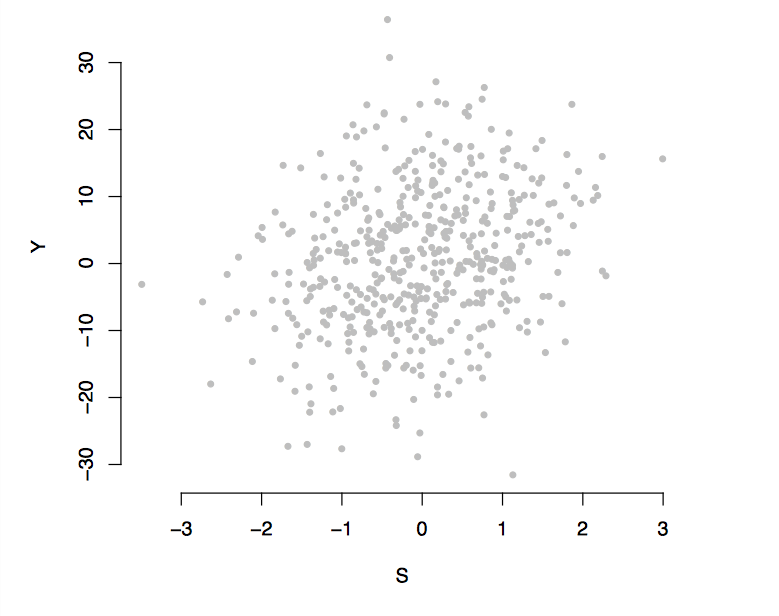
\includegraphics{Figure1.png}}}
\only<2>{\scalebox{0.25}{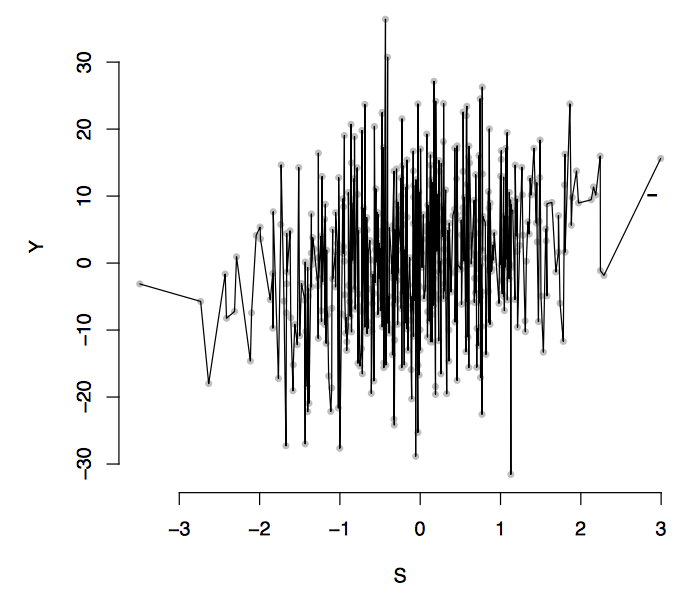
\includegraphics{Figure2.png}}}
\only<3>{\scalebox{0.25}{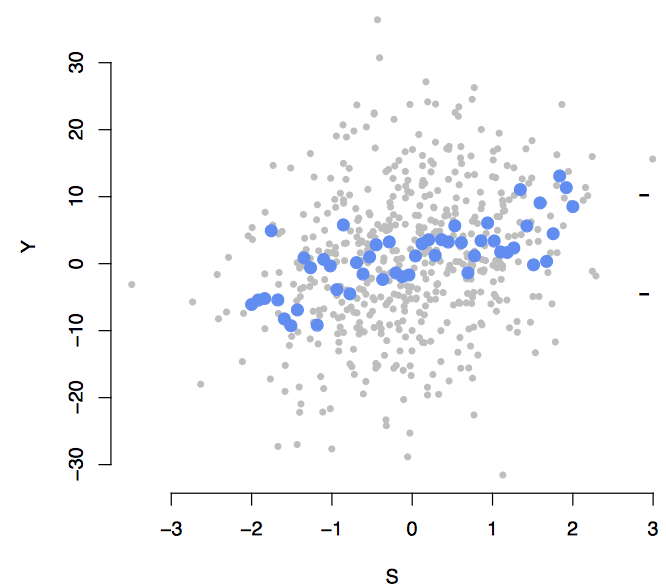
\includegraphics{Figure3.png}}}
\only<4>{\scalebox{0.25}{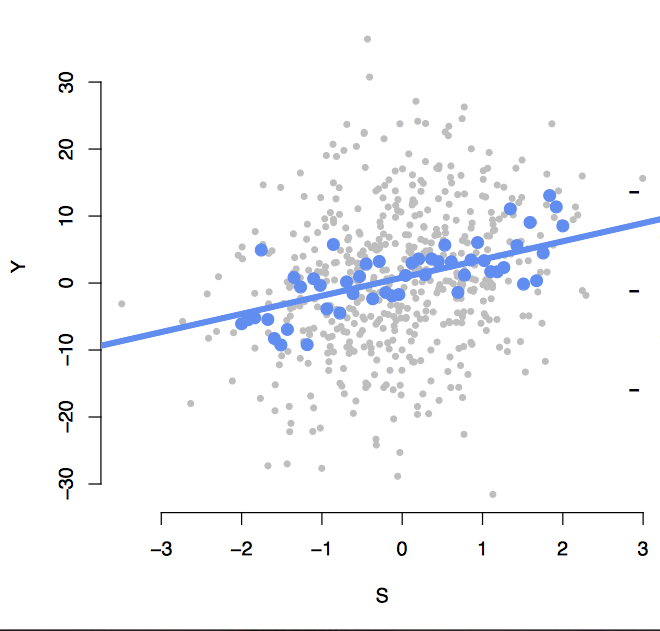
\includegraphics{Figure4.png}}}

\column{0.5\textwidth}
\begin{itemize}
\invisible<1>{\item[-] $E[Y|S]$ with no stratification: every point is in its own ``bin"} 
\invisible<1-2>{\item[-] $E[Y|S]$ after binning the data--no assumed relationship} 
\invisible<1-3>{\item[-] $E[Y|S] = \beta_{0} + \beta_{1} S_{i} $} 
\end{itemize}

\end{columns}
\pause \pause \pause 

\end{frame}



\begin{frame}

For every random variable $Y$ and $S$ we can always write the random variable as, \pause 
\begin{eqnarray}
\invisible<1>{Y_{i} & = & \underbrace{Y_{i} - E[Y|S]}_{\epsilon_{i}} + E[Y|S] \nonumber \\} \pause 
\invisible<1-2>{Y_{i} & = & E[Y|S] + \epsilon_{i} \nonumber \\} \pause 
\invisible<1-3>{Y_{i} & = & \beta_{0} + \beta_{1}S_{i} + \epsilon_{i}  \nonumber } \pause
\end{eqnarray}
\invisible<1-4>{Where we have used our assumption about $E[Y|S] = \beta_{0} + \beta_{1}S_{i}$} \pause


\invisible<1-5>{We'll define our residuals to be,} \pause
\begin{eqnarray}
\invisible<1-6>{\epsilon_{i} & = & Y_{i} - (E[Y|X] ) \nonumber \\} \pause
\invisible<1-7>{& = & Y_{i} - (\beta_{0} + \beta_{1} S_{i}) \nonumber } \pause
\end{eqnarray}


\invisible<1-8>{We are going to find the  $\beta_{0}^{*}, \beta_{1}^{*}$ that minimize the sum of squared residuals, } \pause
\begin{eqnarray}
\only<10>{\invisible<1-9>{(\beta_{0}^{*}, \beta_{1}^{*}) & = & {\tt argmin}_{\beta_{0}, \beta_{1} } \sum_{i=1}^{N} \epsilon_{i}^2 \nonumber } \pause\\}
\only<11>{\invisible<1-10>{(\beta_{0}^{*}, \beta_{1}^{*}) & = & {\tt argmin}_{\beta_{0}, \beta_{1} } \sum_{i=1}^{N} (Y_{i} - \beta_{0} - \beta_{1} S_{i} )^2 \nonumber } \pause}
\end{eqnarray}




\end{frame}






\begin{frame}

Graphically: 

\begin{columns}[]

\column{0.5\textwidth}
\only<1>{\scalebox{0.3}{\includegraphics{LinReg.png}}}
\only<2>{\scalebox{0.3}{\includegraphics{LinReg2.png}}}

\column{0.5\textwidth}

\large
$\beta_{0}^{*}  = \overline{Y} - \beta^{*}_{1} \overline{S}$\\
\large
$\beta_{1}^{*} = \frac{\sum_{i=1}^{N} (S_{i} - \overline{S})Y_{i} }{\sum_{i=1}^{n} (S_{i} - \overline{S})^2 }$ \\
\large
$\beta_{1}^{*} = \frac{\text{cov}(S, Y )}{var(S) }$ \\
{\tt regress<- lm(Y~S) } 






\end{columns}



\end{frame}

\begin{frame}
\frametitle{How To Interpret a Regression?}
\pause 
\invisible<1>{Suppose (again) dichotomous treatment $T_{i}$ and a host of \alert{covariates} $X_{i1}, X_{i2}, \hdots, X_{iK}$.} \pause \\
\invisible<1-2>{Common to specify, } \pause 
\begin{eqnarray}
\invisible<1-3>{Y_{i} & = & \beta_{0} + \alpha T_{i}  + \beta_{1} X_{1} + \beta_{2} X_{2} + \hdots + \beta_{K}X_{k} + \epsilon_{i} \nonumber } \pause
\end{eqnarray}

\begin{itemize}
\invisible<1-4>{\item[-] $\alpha$ is an estimate of the ATE} \pause
\invisible<1-5>{\item[-] $\alpha$ will be a consistent estimate of ATE (converge in probability) if there are no \alert{omitted variables}} \pause
\invisible<1-6>{\item[-] $\alpha$ will be a consistent estimate of ATE (converge in probability) if treatment is as good as randomly assigned, given model} \pause
\begin{itemize}
\invisible<1-7>{\item[1)] $X$'s are \alert{pre-treatment} (not consequences of treatment)} \pause
\invisible<1-8>{\item[2)] We know the $X$'s that are related to treatment assignment + outcome} \pause
\invisible<1-9>{\item[3)] The linear model is right (not more complex functional forms)} \pause
\end{itemize}
\end{itemize}
\invisible<1-10>{\alert{You get one causal effect per regression}:} \pause
\begin{itemize}
\invisible<1-11>{\item[-] The whole point of the $X$'s is \alert{just} to replicate experimental conditions} \pause
\invisible<1-12>{\item[-] \alert{Not} to estimate separate causal effects} 
\end{itemize}


\end{frame}

\end{document}